\section{課題}

\subsection{銅薄膜結晶組織の作成方法依存法について}
小型デバイスの配線パターンの形成技術の一つであるダマシン法について説明する.図\ref{fig:ダマシン}にダマシン法の工程図を示す.まずSiO$_2$等のエッチングしやすい絶縁膜の層に溝を作る.次に電解めっきでその上にCuの膜をつける.その後CMP装置で上部のCuを削り取ると,SiO$_2$層の溝の中にあるCuのみが残り,配線パターンが形成される.Cu配線をドライエッチングでつくることもできるが,反応速度が遅く,十分な生産性が得られないため,ダマシン法が採用される.
\begin{figure}[htbp]
    \centering %中央揃え
    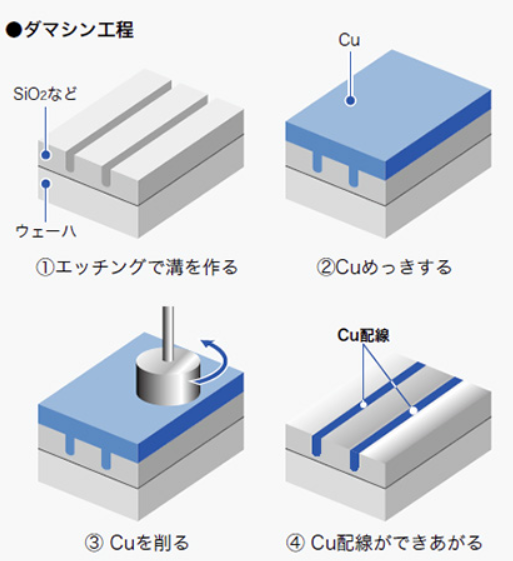
\includegraphics[width=100truemm,clip]{fig/fig_ダマシン.png}
    \caption{Process Diagram of Damascene Method\cite{ダマシン}.}
    \label{fig:ダマシン}
\end{figure}
\subsection{高Crフェライト鋼の微細組織と強度の関係について}
マルテンサイト変態とは,「母相の隣り合う原子が別個に動くのではなく,互いに連携を保ちながらせん断変形的に移動し,新しい結晶構造に変化する変態」のことで,無拡散変態とかせん断型変態ともいう\cite{マルテンサイト}.鋼を高温に熱し,十分な拡散が起きない速さで冷却すると,オーステナイトのFe原子が移動することなく,炭素が体心立方格子の一軸を引き延ばして,一部分に入り込んだ結晶構造に瞬時に変化する.これがマルテンサイト変態の発現機構である.
マルテンサイト変態は無拡散変態であるため,マルテンサイト晶の大きさは母相結晶粒よりも小さい.したがって,結晶粒微細化強化がもたらされ,硬さが向上する.またマルテンサイト晶内には,一般に転位など多くの格子欠陥が導入されているため転位強化が生じ,さらに母相が固溶体であれば,固溶強化もはたらく.実用鋼の場合にはマルテンサイト変態温度が室温以上と高いため,マルテンサイト変態後の室温までの冷却中に炭素の再配列,炭化物の析出などが起こる結果,析出強化も働く.以上のようにマルテンサイトには多くの強化機構が働くため,高強度・高硬度を有する.
\subsection{オーステナイト系ステンレス鋼の鋭敏化について}
SUS304や316などのオーステナイトステンレス鋼が特定の熱履歴を受けると鋭敏化とよばれる粒界でのCr炭化物やCr欠乏層が形成され,耐粒界腐食性が低下する.図\ref{fig:鋭敏化}に鋭敏化発生条件の模式図を示す.およそ600$^\circ$Cから800$^\circ$Cの範囲で,30分ほどの最も短時間で鋭敏化が進行する.低温側の500$^\circ$Cから600$^\circ$Cの範囲では,長時間保持することで鋭敏化し,高温側では長時間保持することで鋭敏化が回復する特徴がある.
鋭敏化が生じる製造過程としては直接ステンレスを熱する溶接や熱処理などが考えられる.またステンレスは熱伝導性が低く,硬い難削材であるため,切削時の摩擦熱による鋭敏化も考えられる.
\begin{figure}[htbp]
    \centering %中央揃え
    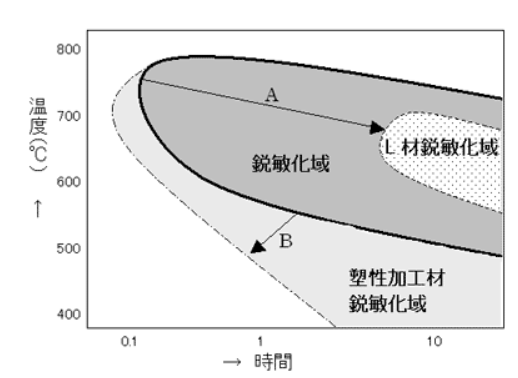
\includegraphics[width=100truemm,clip]{fig/fig_鋭敏化曲線.png}
    \caption{Schematic Diagram of Sensitization Occurrence Conditions\cite{鋭敏化}.}
    \label{fig:鋭敏化}
\end{figure}
\clearpage
